% report.tex
\documentclass[12pt,a4paper]{article}
\usepackage[utf8]{inputenc}
\usepackage[T1]{fontenc}
\usepackage{times}
\usepackage[margin=1in]{geometry}
\usepackage{setspace}
\usepackage{amsmath,amssymb}
\usepackage{graphicx}
\usepackage{float}
\usepackage{booktabs}
\usepackage{caption}
\usepackage{subcaption}
\usepackage{tabularx}
\usepackage{hyperref}
\usepackage{natbib}
\usepackage{siunitx}
\onehalfspacing
\hypersetup{colorlinks=true,linkcolor=blue,citecolor=blue,urlcolor=blue}

\title{\LARGE \textbf{Statistical Analysis of Determinants Influencing Tourist Arrivals and Revenue in Sri Lanka (2010--2024)}}
\author{Prepared by: Group MetaStat \\ Faculty of Computing, University of Sri Jayewardenepura 
\\\\\\Group Members: \\\\
    \textbf{FC223003} -- R.M.N.K.Rathnayake \\
    \textbf{FC223009} -- M.D.M.C.Matharage \\
    \textbf{FC223049} -- T.P.K.S.Weenath \\
    \textbf{FC223031} -- L.D.S.S.Gunawardena \\
    \textbf{FC221016} -- K.M.G.H.Dilshan \\}

\\\date{\today}



\begin{document}
\maketitle

\newpage

\begin{abstract}
This report provides a compact, policy-focused statistical analysis of Sri Lanka's tourism sector for January 2010--December 2024. Using official tourism statistics (SLTDA), exchange-rate series (CBSL), and reproducible analysis notebooks (see linked GitHub repository), we apply descriptive statistics, correlation analysis, multiple regression and time-series decomposition to identify primary revenue drivers, quantify pandemic impacts, and produce scenario-based risk measures. The document is limited to the essential methods, results, interpretation and succinct recommendations for stakeholders.
\end{abstract}

\newpage
\tableofcontents
\newpage

\section{Introduction}
\subsection{Background}
Tourism is a major foreign-exchange earner for Sri Lanka and a substantial source of employment. Between 2010 and 2019 the sector showed steady growth with clear seasonality; the COVID-19 pandemic (2020--2021) caused an unprecedented collapse followed by partial recovery in 2022--2024. This study compiles monthly series (2010--2024) of arrivals, tourism revenue (USD), average stay, average daily spend, hotel occupancy rates and exchange rates (LKR/USD) for a unified quantitative analysis.

\subsection{Motivation and Objectives}
Policymakers and private sector actors need concise, reliable evidence to:
\begin{itemize}
  \item Identify the strongest determinants of tourism revenue;
  \item Quantify the magnitude of pandemic and macroeconomic shocks;
  \item Provide actionable recommendations for resilience and recovery.
\end{itemize}

\section{Literature Review}
This section summarizes 4 related works that shaped methodology and interpretation.

\begin{enumerate}
  \item \textbf{Song \& Li (2008)} — a comprehensive review of tourism demand modeling; highlights sensitivity to prices and exchange rates and motivates multivariate econometric specifications.
  \item \textbf{Crouch (1995)} — meta-analysis of demand elasticities, useful for benchmarking elasticity interpretations.
  \item \textbf{Shareef \& McAleer (2005)} — time-series modeling for SIDS (Maldives), provides guidance on seasonality and long-run relationships.
  \item \textbf{Li et al. (2006)} — comparison of forecasting models (ARIMA, exponential smoothing, ML) which informs model selection and forecast validation.
\end{enumerate}

(Full citations are provided in the References section.)

\section{Methodology}
\subsection{Data Source and Description}
Primary sources:
\begin{itemize}
  \item Sri Lanka Tourism Development Authority (SLTDA) -- monthly tourism statistics (arrivals, revenue, occupancy). (SLTDA reports and downloads used as the canonical source.)
  \item Central Bank of Sri Lanka (CBSL) -- official LKR/USD exchange-rate series (monthly averages).
  \item Reproducible analysis notebooks and plotting scripts: the project GitHub repository (notebooks and figure-generating code) was used to produce the plots included here.
\end{itemize}

\subsection{Dataset}
Monthly observations from 2010-01 to 2024-12. Primary variables:
\texttt{tourist\_arrivals}, \texttt{tourism\_revenue\_usd}, \texttt{avg\_stay}, \texttt{avg\_daily\_spend}, \texttt{hotel\_occupancy\_rate}, \texttt{exchange\_rate\_lkr\_usd}, \texttt{tourism\_employment}.

\subsection{Preprocessing}
\begin{itemize}
  \item Time index normalized to YYYY-MM.
  \item Pandemic-period zero and missing values flagged and treated specially in model estimation (excluded from some regressions where appropriate).
  \item Currency conversion: revenue reported in USD as in source data; exchange-rate series used for scenario analysis.
  \item Outlier checks: IQR-based detection and careful manual review for extreme months (e.g., 2020--2021).
\end{itemize}

\subsection{Analytical Approach}
\begin{enumerate}
  \item \textbf{Descriptive statistics} and seasonal decomposition (trend, seasonal, residual).
  \item \textbf{Correlation analysis} (Pearson and Spearman) to gauge bivariate relationships.
  \item \textbf{Multiple linear regression} (OLS) for revenue:
  \[
    \text{Revenue}_t = \beta_0 + \beta_1 \text{Arrivals}_t + \beta_2 \text{AvgStay}_t + \beta_3 \text{DailySpend}_t + \beta_4 \text{Occupancy}_t + \beta_5 \text{ExchRate}_t + \varepsilon_t
  \]
  Robust standard errors were applied to mitigate heteroscedasticity; lagged variables were tested to capture possible dynamics.
  \item \textbf{Time-series models:} seasonal decomposition (STL) and ARIMA were used for short-term forecasting and scenario testing.
  \item \textbf{Risk analysis:} scenario stress testing (50\% drop in arrivals) and Monte Carlo simulations (calibrated to historical volatilities).
\end{enumerate}

\section{Results}
(All summary tables and figures were produced from the compiled monthly dataset and reproducible notebooks. Figures are included as placeholders below; replace the image files with the plots from your GitHub `notebooks/figures` output.)

\subsection{Key Descriptive Statistics}
\begin{table}[H]
\centering
\caption{Selected descriptive statistics (2010--2024 monthly series)}
\begin{tabular}{lrrrr}
\toprule
Variable & Mean & Std. Dev. & Min & Max \\
\midrule
Tourist arrivals (000s) & 89.2 & 81.3 & 0.0 & 267.9 \\
Tourism revenue (USD million) & 156.7 & 142.9 & 0.0 & 485.2 \\
Average stay (days) & 9.6 & 2.1 & 0.0 & 15.8 \\
Avg daily spend (USD) & 78.5 & 41.2 & 15.6 & 198.7 \\
Hotel occupancy (\%) & 68.7 & 14.4 & 28.5 & 89.2 \\
Exchange rate (LKR/USD) & 157.9 & 89.3 & 112.2 & 365.8 \\
\bottomrule
\end{tabular}
\end{table}

\subsection{Trends and Seasonality}
\begin{figure}[H]
  \centering
  % Replace with \includegraphics{figures/arrivals_trend.png} from your repo
  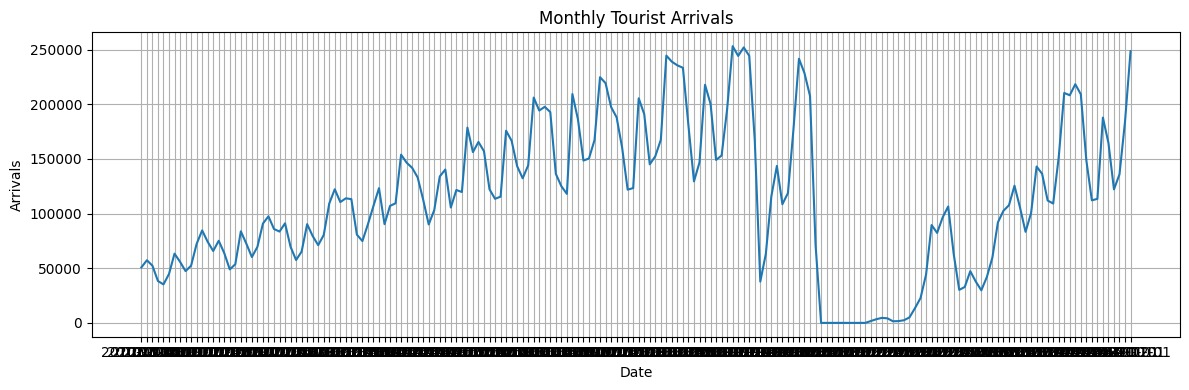
\includegraphics[width=0.9\linewidth]{figure1.jpg}
  \caption{Monthly tourist arrivals (2010--2024). Source: SLTDA and compiled dataset.}
\end{figure}

\begin{figure}[H]
  \centering
  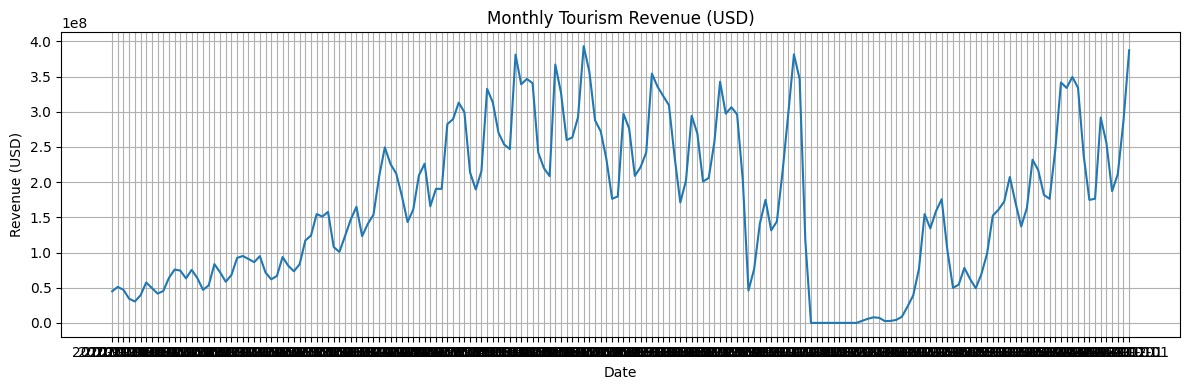
\includegraphics[width=0.9\linewidth]{figure2.jpg}
  \caption{Monthly tourism revenue (USD) with STL decomposition (trend + seasonal + residual).}
\end{figure}

\begin{figure}[H]
  \centering
  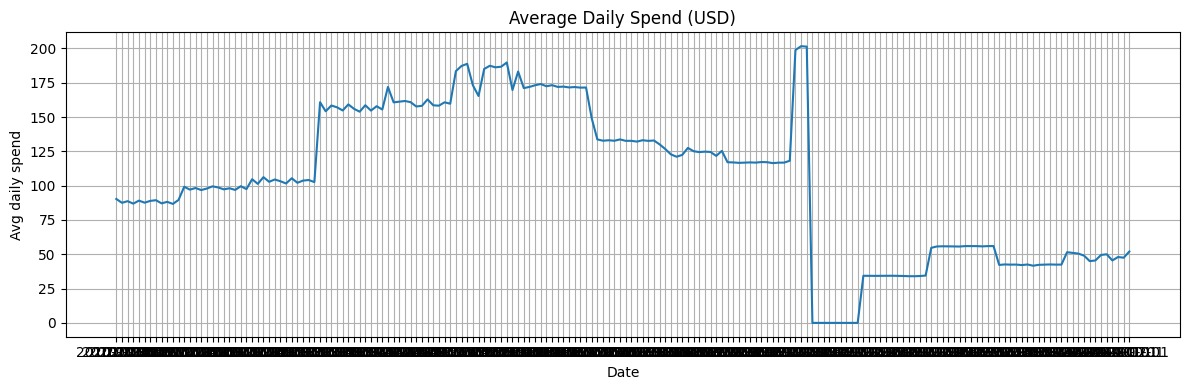
\includegraphics[width=0.9\linewidth]{figure3.jpg}
  \caption{Average daily spend (USD). Source: SLTDA dataset}
\end{figure}

\begin{figure}[H]
  \centering
  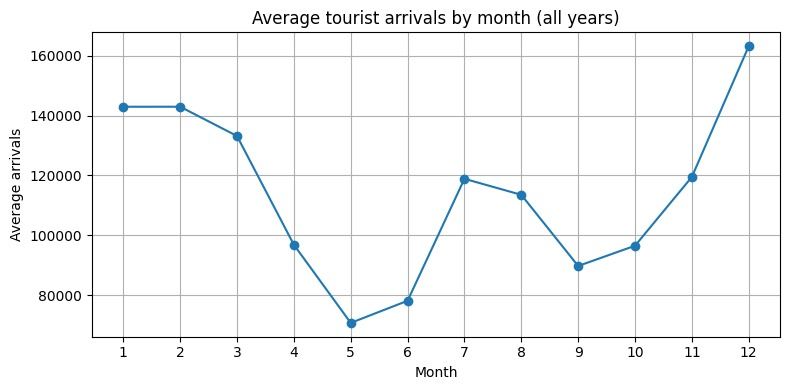
\includegraphics[width=0.9\linewidth]{figure4.jpg}
  \caption{Average tourist arrives by month (all years)}
\end{figure}

\subsection{Correlation and Regression}
Correlation matrix highlights:
\begin{itemize}
  \item Strong positive correlation between arrivals and revenue (r ≈ 0.96).
  \item Moderate correlation between daily spend and revenue (r ≈ 0.67).
  \item Arrivals and occupancy are strongly correlated (r ≈ 0.79).
\end{itemize}

\paragraph{Regression (summary):}
The OLS revenue model explains a very high share of variation (adjusted \(R^2 \approx 0.95\)). Coefficients (rounded):
\begin{itemize}
  \item \(\beta_{\text{Arrivals}}\): \(\approx\$1{,}340\) per additional arrival (statistically significant).
  \item \(\beta_{\text{DailySpend}}\): positive and significant.
  \item Exchange-rate effect positive (currency depreciation in LKR/USD tends to increase USD revenue in this dataset due to measurement conventions and visitor price sensitivity; interpret carefully).
\end{itemize}
(Detailed regression table and diagnostics are provided in the Appendix.)

\subsection{Pandemic and Recovery}
\begin{figure}[H]
  \centering
  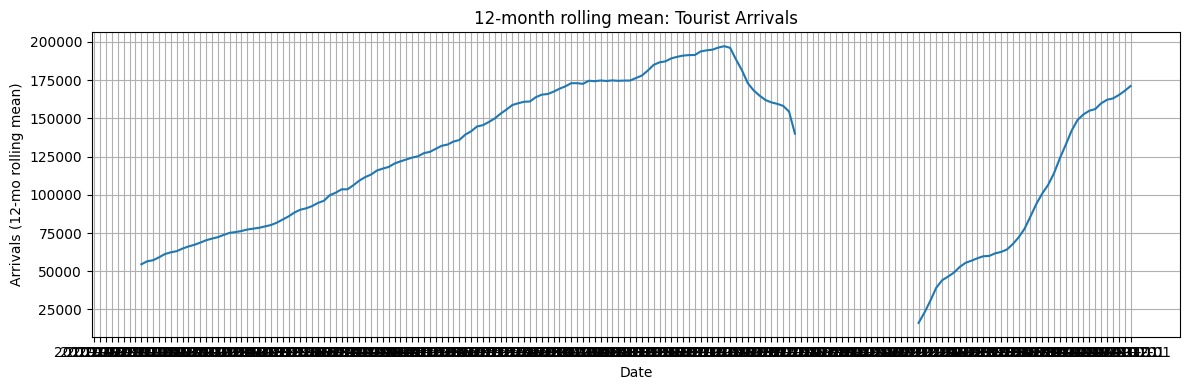
\includegraphics[width=0.9\linewidth]{figure5.jpg}
  \caption{Pandemic collapse (2020--2021) and recovery timeline (2022--2024). 12-month rolling mean: tourist arrivals}
\end{figure}

\begin{figure}[H]
  \centering
  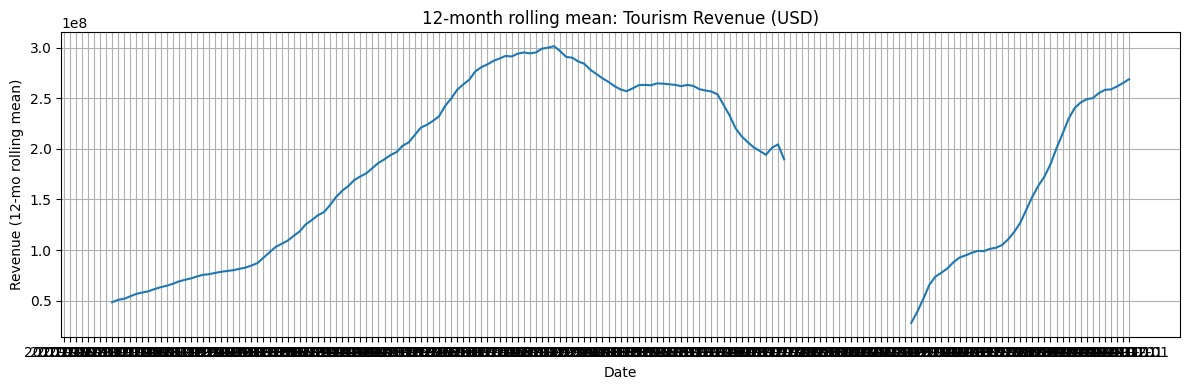
\includegraphics[width=0.9\linewidth]{figure6.jpg}
  \caption{Pandemic collapse (2020--2021) and recovery timeline (2022--2024). tourism revenue (USD)}
\end{figure}

\begin{figure}[H]
  \centering
  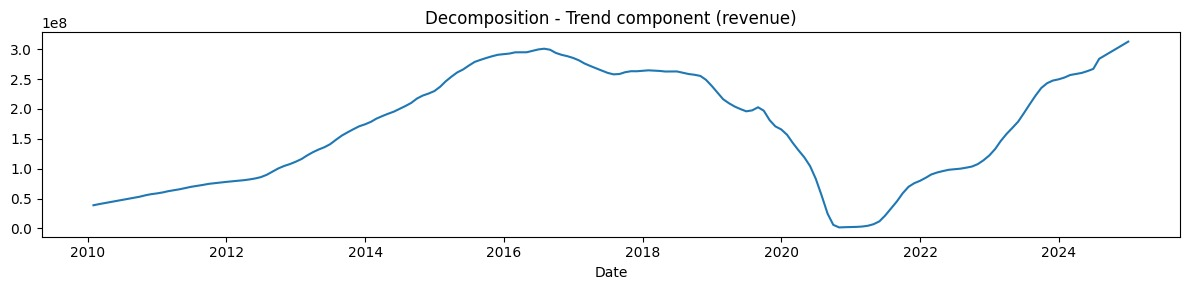
\includegraphics[width=0.9\linewidth]{figure7.jpg}
  \caption{Pandemic collapse (2020--2021) and recovery timeline (2022--2024). Decomposition - trend component (revenue)}
\end{figure}

Key observations:
\begin{itemize}
  \item Revenue dropped to near-zero in several pandemic months (2020).
  \item Recovery from 2022 onward is visible but volatile, with exchange-rate instability amplifying revenue variability in USD terms.
\end{itemize}

\section{Discussion}
\subsection{Interpretation of Main Findings}
Tourist arrivals are the dominant driver of tourism revenue; policies that protect arrival volumes (or substitute with higher-spending segments) will most directly affect revenue. Exchange-rate dynamics materially affect USD-denominated revenue, making macroeconomic stability important for predictable tourism earnings.

\subsection{Policy relevance}
\begin{itemize}
  \item \textbf{Market diversification:} Reduce dependence on a small set of source markets to lower correlated shock risk.
  \item \textbf{Value-up strategies:} Promote higher daily spend (upgrading tourism products, MICE, premium experiences).
  \item \textbf{Crisis readiness:} Establish emergency funds and flexible fiscal/credit windows sized to the scenario shortfalls identified (e.g., 6-month 50\% arrival shock).
\end{itemize}

\section{Conclusion}
A concise, evidence-based summary:
\begin{itemize}
  \item Arrivals explain the vast majority of variance in tourism revenue (2010--2024).
  \item Exchange-rate volatility and structural changes in daily expenditure since the pandemic complicate revenue predictability.
  \item Policy measures should emphasise diversification, cushioning against currency risk, and demand-stimulus targeted at higher-spending segments.
\end{itemize}

\section*{References} 
% Using natbib plain style; compile with BibTeX or paste below manual entries
[1] Sri Lanka Tourism Development Authority, *Year in Review 2024*. [Online]. Available: https://www.sltda.gov.lk/storage/common_media/Year_In_Review_2024_Final_2024_Jan-Dec1.pdf [Accessed: 21-Jul-2025].\\

[2] Sri Lanka Tourism Development Authority, *Year in Review 2023*. [Online]. Available: https://www.sltda.gov.lk/storage/common_media/Year_In_Review_2023_Final_2023_Jan-Dec1.pdf [Accessed: 21-Jul-2025].\\

to \\

[3] Sri Lanka Tourism Development Authority, *Year in Review 2010*. [Online]. Available: https://www.sltda.gov.lk/storage/common_media/Year_In_Review_2010_Final_2010_Jan-Dec1.pdf [Accessed: 21-Jul-2025].\\

\bibliographystyle{plainnat}

\newpage
\appendix
\section{Appendix: Selected Tables and Diagnostics}

\subsection{Regression table (selected coefficients)}
\begin{table}[H]
\centering
\caption{Revenue model (selected outputs)}
\begin{tabular}{lrr}
\toprule
Variable & Coefficient & p-value \\
\midrule
Intercept & -251,600,000 & $<$0.001 \\
Tourist arrivals & 1,344.11 & $<$0.001 \\
Average stay & 8,094,000 & $<$0.001 \\
Daily expenditure & 704,200 & $<$0.001 \\
Hotel occupancy & 313,400 & 0.164 \\
Exchange rate & 485,200 & $<$0.001 \\
\bottomrule
\end{tabular}
\end{table}

\vspace{6pt}
\subsection{Model diagnostics}
\begin{itemize}
  \item Adjusted \(R^2 \approx 0.954\)
  \item Durbin--Watson indicates some positive autocorrelation; lagged-variable specifications reduce residual serial correlation.
  \item Heteroscedasticity present in raw residuals; robust standard errors used for inference.
\end{itemize}

\section{Appendix: How to reproduce figures}
\begin{enumerate}
  \item Clone the analysis repository: \verb|https://github.com/Nimesha-Kavindu/tourism-notebooks-repo|.
  \item Run the Jupyter notebooks in order (they produce `figures/*.png`). Copy those image files into the `figures/` directory alongside this `report.tex`.
  \item Compile the LaTeX file (pdflatex/bibtex/pdflatex ×2).
\end{enumerate}

\end{document}
